%!TEX root = FreeRtos ARM uController.tex

%\subsection{Anforderung Desktop Betriebssystem vs. Anforderung Echtzeit Betriebssystem}
%Desktop Betriebssysteme verwalten den Hardwarezugriff und stellen sicher, dass eingesetzte Software die benötigte Rechenzeit zur Verfügung gestellt bekommt. Gleichzeitig regeln Sie den Hardwarezugriff und organisieren den konkurrierenden Zugriff, beispielsweise auf Netzwerkkarten und Festplatten. Sie stellen Funktionen für die Interprozesskommunikation bereit und übernehmen grundlegende Aufgaben wie die Organisation von Arbeitsspeicher. Im Gegensatz zu einem gewöhnlichen Desktop Betriebssystem liegt der Anwendungsfokus bei Echzeit Betriebssystemen nicht auf der direkten Userinteraktion. Die wenigsten Echtzeitbetriebssysteme bieten eine Benutzeroberfläche. Die Interaktion mit der Umwelt geschieht durch spezielle Hardware und ist zumeist für genau eine Aufgabe ausgelegt. Viele Funktionen die eine Desktop Betriebssystem übernimmt wie z.B. das Verwalten von konkurrierenden Zugriffen auf externe Geräte müssen vom Entwickler selbst übernommen werden. Ein Echtzeitbetriebssystem bietet bei weitem nicht die Funktionalitäten eines Desktop Betriebssystems, das liegt zum Einen an der Art von Zielsystemen, die zumeist nur einen beschränkten Speicher aufweisen und Zweitens an der Tatsache das die vom Echtzeitbetriebssystem bereitgestellten Funktionen deterministisch sein müssen.   
%
%WIP: Gefällt insgesamt noch nicht, benötigen wir Anforderungen an ein Destkop Betriebssystem ?? Echzeitbetriebsysteme unterscheiden sich erheblich von normalen Betriebssystemen. Wie schon angesprochen verwaltet ein RTOS nur die Zeit (Scheduler) + Speicher (Memory Allocation) 
%
\subsection{Echtzeitsysteme und Echtzeitbetriebssysteme}
Mit der steigenden Leis\-tungs\-fähig\-keit von modernen $\mu$\-Pro\-zesso\-ren, steigen auch die Anforderungen an die Software die auf diese Systeme aufsetzt. Viele dieser Systeme verlangen trotz ihrer Komplexität, dass Teile des Programmablauf in bestimmten zeitlichen Grenzen ausgeführt wird und somit vorhersehbar und deterministisch sind. Systeme die eine solche Anforderung unterliegen werden Echtzeitsysteme genannt. Echtzeitsysteme unterliegen einer weiteren Unterteilung in weiche Echtzeitsystem (soft realtime systems) und harte Echtzeitsysteme (hard realtime systems). Ein weiches Echtzeitsysteme soll eine Aufgabe in den vorgegeben zeitlichen Grenzen ausführen, ein über\-schreiten ist aber erlaubt und führt nicht unmittelbar zu einem Fehler. Ein hartes Echtzeitsystem hingegen muss die gestellte Aufgabe in den vorgegebenen Grenzen aus\-füh\-ren. Eine Überschreitung macht das System unbrauchbar. Einige Beispielsysteme und deren Echtzeitzuordnung wir in Tabelle \ref{tab:BeispieleEchzeitsystem} gezeigt. Um die grundsätzliche Funktionalität eines Echtzeitbetriebssystems zu erläutern, müssen zu erst die Grundmodelle für den Programmablauf eingebetter Systeme beschrieben werden. Der Programmablauf eingebetteter Systeme lässt sich auf drei Modelle zurückführen (Abbildung \ref{fig:Programmablauf}). Eingebettete Anwendungen können in einer einzigen Schleife (mit oder ohne Interrupt Unterbrechungen) laufen oder aber in event-gesteuerten ne\-ben\-läuf\-igen ei\-gen\-stän\-dig\-en Programmabschnitten (Thre\-ad oder Task\footnote{Nachfolgenden wird Task benutzt, da dies der geläufige Begriff bei FreeRTOS ist. In der Literatur zu Echtzeitsystemen ist der Begriff nicht exakt definiert.}) ausgeführt werden. Die nebenläufige Aus\-füh\-rung der unterschiedlichen Programmsegmente ist nur durch einen RTOS-Kernel (Scheduler) zu erreichen. Ein RTOS Kernel abstrahiert Timing Informationen und küm\-mert sich darum, dass die nächste Task rechtzeitig ausgeführt wird. Der Entwickler ist dafür verantwortlich, dass die Task die gewünschte Aufgabe im zeitlichen Rahmen ausführt. Wie sichergestellt werden kann, dass eine Task  harten oder weichen Echtzeitanforderungen entspricht wird Abschnitt \ref{sec:Echtzeitanalyse} beschrieben. Für viele kleine Anwendungen kann die Nutzung einer einzigen Schleife durchaus sinnvoll sein, sollten beispielsweise die Ressourcen so knapp sein, dass ein Overhead an Funktionalität ausgeschlossen werden muss. Ein großer Nachteil der "`einschleifen Variante"' ist die permanente Nutzung des Prozessors. Besonders bei akkubetriebenen Geräten wie IoT Devices oder Mobiltelefonen wird sehr genau auf die Energieaufnahme geachtet. Ein RTOS bietet hingegen Funktionen mit denen sehr leicht ermittelt werden kann, ob ein Gerät in einen Schlafmodus wechseln kann, dies wird in Abschnitt \ref{sec:Low Power Modes} an Beispielen von FreeRTOS und einem ARM $\mu$Prozessor demonstriert. Neben der Echtzeitfähig gibt es aber noch viele weitere Vorzüge für den Einsatz eines Echtzeitbetriebssystems.  
Durch das Herunterbrechen der Anwendung in Task entstehen viele kleine Module, die jeweils eine kleine Teilaufgabe des Gesamtsystems übernehmen.Durch ein sauber definiertes Interface zur Kommunikation der Tasks, lässt sich die Entwicklungsarbeit leicht auf mehrere Teams verteilen. Dies ermöglicht auch den Einsatz von agilen Entwicklungsmethoden wie Scrum in der Entwicklung von eingebetteten Systemen. 
To be continued ... ;)  
\newline  
\begin{figure}
	\centering
		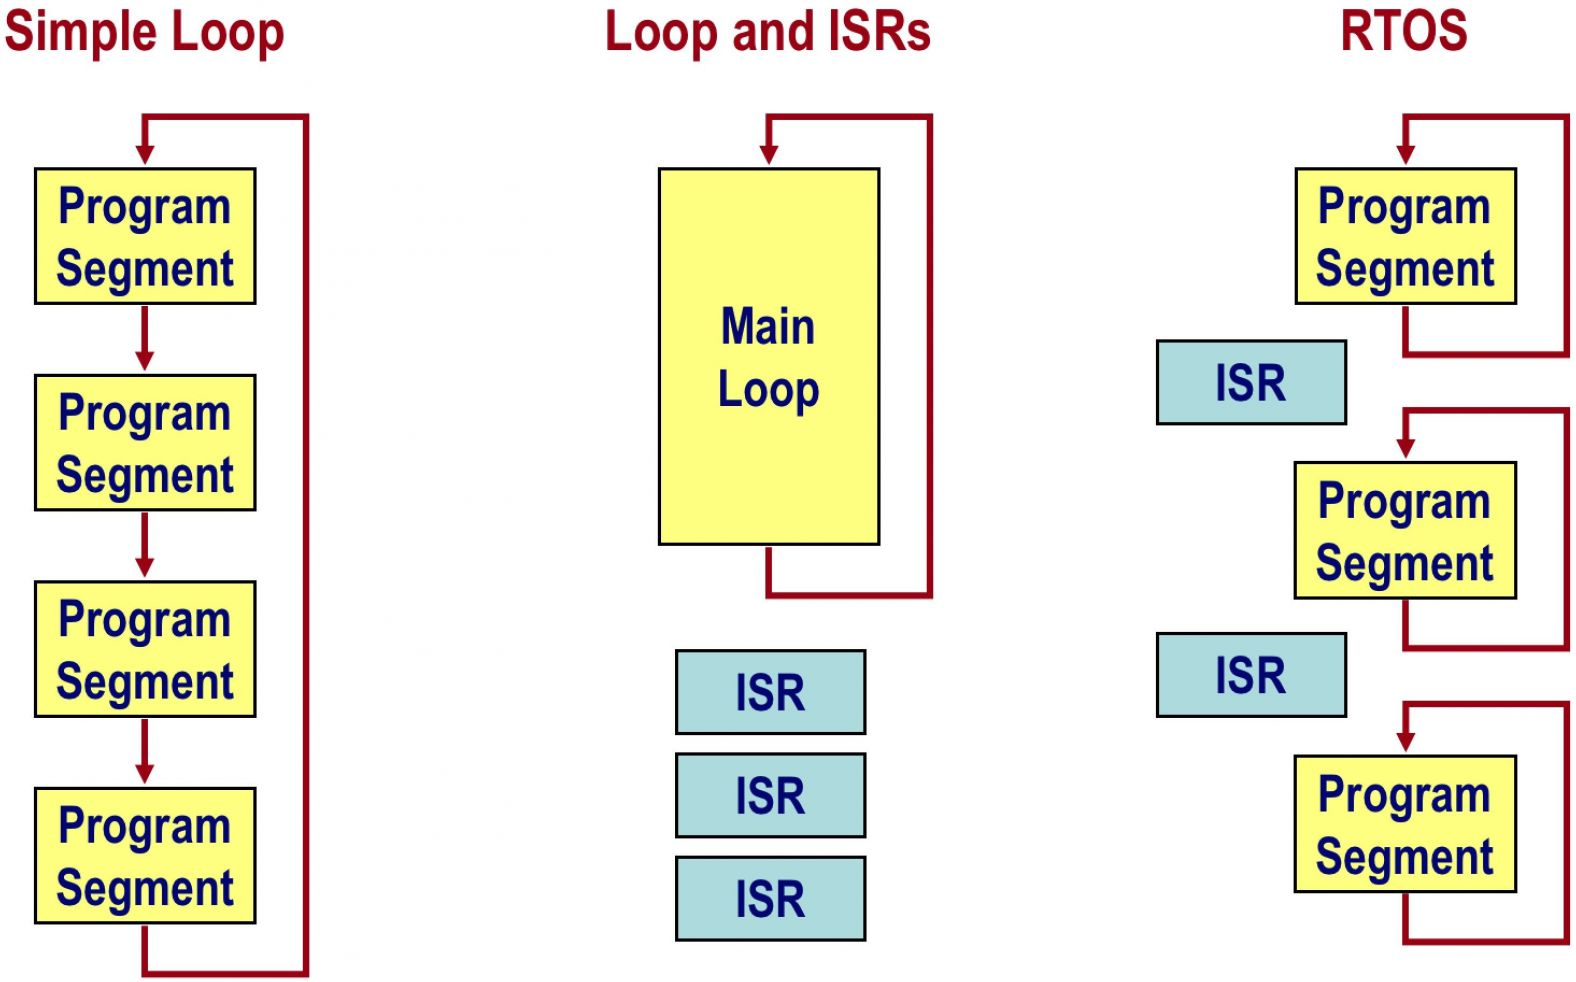
\includegraphics[width=0.3\textwidth]{Pictures/EmbeddedCom/cwrtos2f5c.jpg}
	\caption{Übersicht Programmabläufe in embedded Anwendungen. Quelle~\protect\citeA{RTOSRevealed}}
	\label{fig:Programmablauf}
\end{figure}

\begin{table*}
\centering
	\begin{tabular}{|l|l|l|}
		\hline
		\textbf{Beispiel} & \textbf{Echtzeit Typ}  & \textbf{Auswirkung} \\
		\hline
		Tastatur Controller & Soft Realtime & kurzfristig verzögerte Ausgabe \\
		\hline
		Echtzeit Media Streaming  & Soft Realtime & Bild und Ton kurzfristig asynchron \\
		\hline
		Controller CD Laufwerk  & Hard Realtime & Fehler beim Lesen\\
		\hline
		Airbag System  & Hard Realtime & möglicher Personenschaden\\
		\hline
	\end{tabular}
	\caption{Beispiele Echzeitsystem}
	\label{tab:BeispieleEchzeitsystem}
\end{table*}




%Echtzeitbetriebssysteme kommen zum Einsatz wenn neben den oben genannten Anforderungen an ein normales Betriebssystem weitere Anforderungen gestellt werden, die ein normales Betriebssystem nicht berücksichtigt. Dies können beispielsweise garantiert berechenbare Reaktionszeiten sein wie sie in der Fabrikation oder im Automobilbereich gefordert werden oder geringe Leistungsaufnahmen wie bei Komponenten des Internet of Things (IoT). Insgesamt wird zwischen Harten und Weichen Echtzeitkriterien unterschieden. Diese Gliedern sich wie folgt:\newline
%Aufgrund der Eingangs geschilderten Einsatzbereiche ist leich zu erkennen, dass Echzeitbetriebssysteme häufigin Umgebungen zum Einsatz kommen, in denen besondere Anforderungen an die Hardware gestellt werden. Häufig verfügt die Hardware nur über begrenzte Speicherkapazitäten, über geringe Wärmeableitfähigkeiten und damit geringe Rechenleistung. Die zur Verfügung stehende Energie muss bei der Entwicklung ebenfalls berücksichtigt werden. 
%Vor diesem Hintergrund benötigen Echtzeitbetriebssysteme nur wenig Speicherplatz und implementieren Funktionen um den Prozessor und die angeschlossene Peripherie nur kurzzeitig zu belasten und in der restlichen Zeit in den Ruhezustand zu verseten.
